\documentclass[10pt]{beamer}

\usepackage[american]{babel}
\usepackage[utf8]{inputenc}
\usepackage{soul}
\usepackage{amsmath}
\usepackage{amssymb}
\usepackage{listings}
\lstset{
  language=haskell,
  upquote=true,
  basicstyle=\ttfamily,          % print whole listing in typewriter
  keywordstyle=\color{blue}\bfseries, % bold blue keywords
  %identifierstyle=,           % nothing happens
  commentstyle=\color{green}, % green comments
  stringstyle=\color{red},      % typewriter type for strings
  showstringspaces=false     % no special string spaces
}
\usepackage[all]{xy}
\usepackage{tikz}
\usetikzlibrary{arrows,shapes,automata}
\usepackage{graphicx}
\usepackage[bibstyle=beamer,citestyle=authoryear-comp,doi=false,isbn=false,eprint=false,maxnames=10]{biblatex}
\bibliography{../defeo}
\usepackage{../mysymbols}
\usepackage{array}

\usepackage[T1]{fontenc}
\usepackage{textcomp}
\renewcommand{\rmdefault}{pplx}
\renewcommand{\sfdefault}{uop}
\usepackage[T1]{eulervm}


\mode<presentation>{%
  \usetheme[]{Madrid}
  \usefonttheme{professionalfonts}
  \usecolortheme{crane}
% \usecolortheme{rose}
}


\title{Fast algorithms: from type theory to number theory}
\author{Luca~De~Feo}
\institute[INRIA Saclay]{INRIA Saclay, Projet TANC}
\date[INRIA Rocquencourt, October 25, 2010]{October 25, 2010\\Séminaire Algorithmes\\INRIA Rocquencourt, Le Chesnay}


\AtBeginSection[]
{
  \begin{frame}<beamer>
    \frametitle{Plan}
    \tableofcontents[currentsection]
  \end{frame}
}

\begin{document}

\begin{frame}
  \titlepage
\end{frame}

%%
%%

\begin{frame}
  \frametitle{Elliptic curve cryptography}
  
  \begin{columns}
    \begin{column}{0.4\textwidth}
      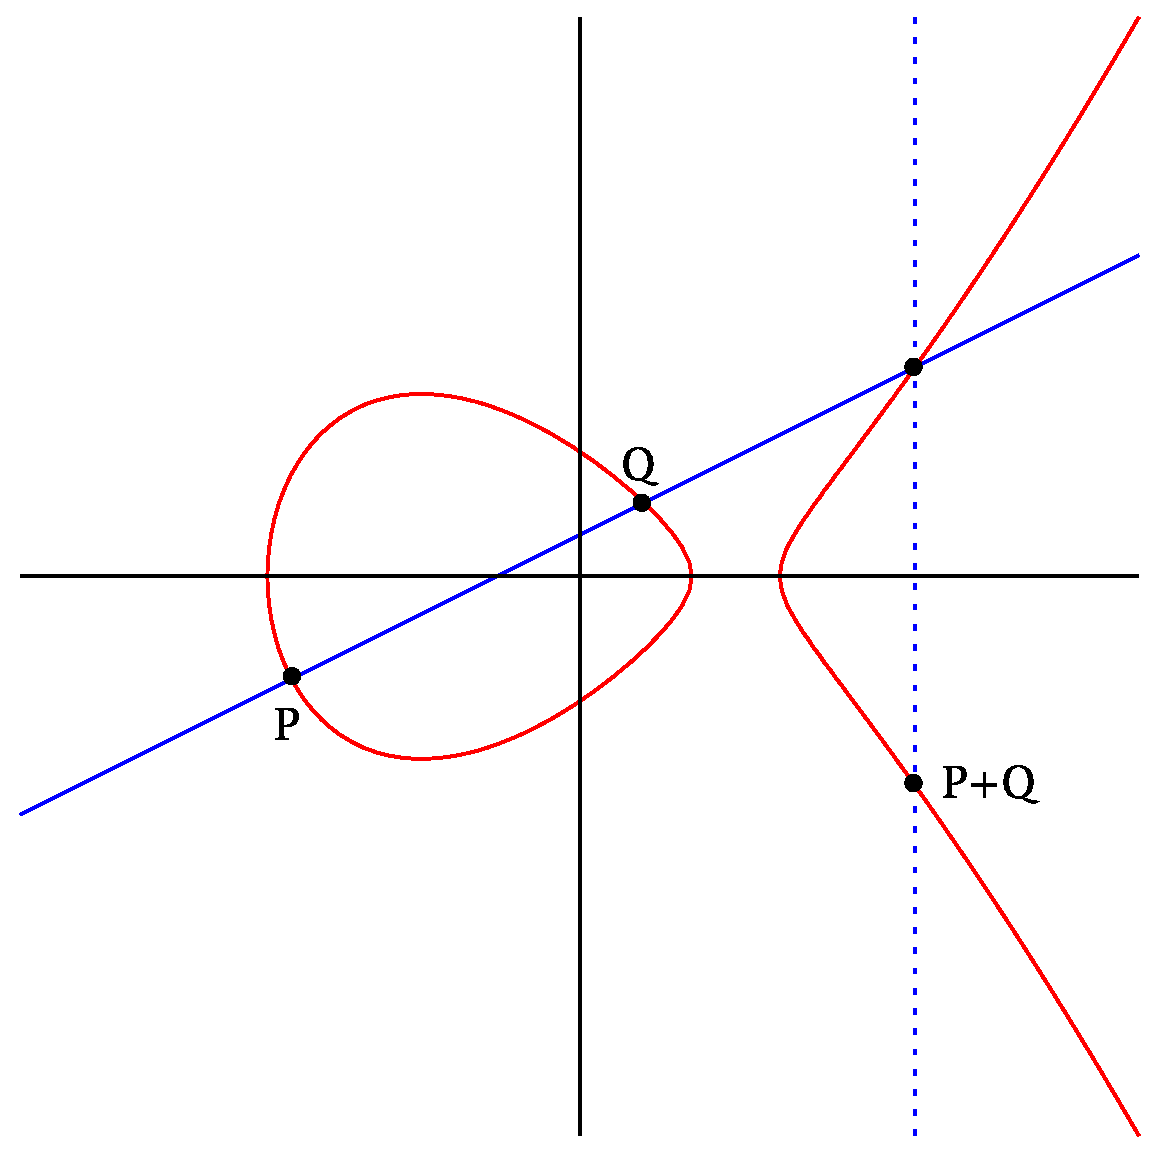
\includegraphics[width=\textwidth]{../isogeny/ec-add.pdf}
    \end{column}
    \begin{column}{0.6\textwidth}
      \begin{description}
      \setlength{\itemsep}{\baselineskip}
      \item[Weierstrass form:] $y^2 = x^3 + ax + b$;
      \item[Group law:] Chord-tangent;
      \item[Crypto:] Based on discrete log in $E(\F_q)$;
      \item[Hasse bound:] $\lvert\card{E}(\F_q) -
        q-1\rvert\le2\sqrt{q}$.
      \end{description}
    \end{column}
  \end{columns}
\end{frame}

%%

\begin{frame}
  \frametitle{Isogenies}
  
  \begin{columns}
    \begin{column}{0.5\textwidth}
      Isogenies are group morphisms of elliptic curves:
    \end{column}
    \begin{column}{0.5\textwidth}
      \begin{align*}
        \I      &:E\ra E'\\
        \I(x,y) &= \left(\frac{g(x)}{h(x)}, cy\left(\frac{g(x)}{h(x)}\right)'\right)
      \end{align*}
    \end{column}
  \end{columns}

  \begin{block}{What do you do with an isogeny over a finite field?}
    \begin{itemize}
    \item Point counting (\cite{schoof95});
    \item Speed up point multiplication (\cite{gallant+lambert+vanstone01});
    \item Reduce a Discrete Logarithm Problem to another (\cite{gaudry+hess+smart02,smith09});
    \item Construct new cryptosystems (\cite{teske06,rostovtsev+stolbunov06});
    \item Construct hash functions (\cite{charles+lauter+goren09}).
    \end{itemize}
  \end{block}
\end{frame}

%%

\begin{frame}
  \frametitle{Isogenies: an example}

  \vspace{-1mm}

  \begin{block}{The GHS attack (\cite{gaudry+hess+smart02})}
    \centering
    $\xymatrix{
      E/F_{q^d} \only<2->{\ar[r]^\I} & \only<2->{H/F_q}
    }$
    \begin{itemize}
    \item Given an elliptic curve $E$ defined over a composite field $\F_{q^d}$;
    \item<2-> Computes an isogeny to an hyperelliptic curve $H$
      defined over $\F_q$.
    \item<2-> For certain parameters, the discrete log is easier on
      $H$ than on $E$.
    \end{itemize}
  \end{block}

  \vspace{-0.3mm}

  \begin{block}<3->{A trapdoor cryptosystem (\cite{teske06})}
    \textbf{Fact:} Only a small fraction of the curves over $\F_{q^d}$
    is vulnerable to GHS

    \centering
    $\xymatrix@R=0pt{
      E_{\mathrm{trap}} \only<4->{\ar[dr]} &         & \only<4->{\ar[dr]} &\\
      & \only<4->{\ar[ur]} &         & \only<4->{E_{\mathrm{pub}}}
    }$
    \begin{itemize}
    \item Select a curve $E_{\mathrm{trap}}$ vulnerable to GHS;
    \item<4-> Take a random walk through the \emph{isogeny graph},
      land on a curve $E_{\mathrm{pub}}$ not vulnerable to GHS;
    \item<5-> Use $E_{\mathrm{pub}}$ for public key cryptography, give
      $E_{\mathrm{trap}}$ to a \emph{trusted authority} for \emph{key
        escrow}.
    \end{itemize}
  \end{block}
\end{frame}

%%

\begin{frame}
  \frametitle{Isogenies: a challenge}
  Let
  \[\F_q = \F_2[Z]/(Z^{41} + Z^3 + 1)\]

  The following two curves are isogenous:
  
  \begin{block}{}
    ${y^2 + xy = x^3 + 1/(Z^{36}} + Z^{35} + Z^{34} + Z^{32} + Z^{31}
    + Z^{30} + Z^{26} + Z^{23} + Z^{22} + Z^{21} + Z^{20} + Z^{18} +
    Z^{17} + Z^{13} + Z^{12} + Z^{11} + Z^8 + Z^7 + Z^5 + Z^4 + Z^2)$
  \end{block}

  \begin{block}{}
    ${y^2 + xy = x^3 + 1/(Z^{40}} + Z^{39} + Z^{38} + Z^{37} + Z^{35}
    + Z^{34} + Z^{28} + Z^{22} + Z^{15} + Z^{14} + Z^{11} + Z^{10} +
    Z^9 + Z^8 + Z^7 + Z^6 + Z^5 + Z^4 + Z)$
  \end{block}
  
  \begin{itemize}
  \item Can you tell of what degree (i.e. size of the kernel)? 
  \item Can you compute the isogeny?
  \end{itemize}
\end{frame}

%%
%%

\section{Transposition principle}

\begin{frame}
  \frametitle{The transposition principle}

  \begin{quote}
    \large ``Let $\pspace$ be an arbitrary set. To any $R$-algebraic
    algorithm $A$ computing a family of linear functions $(f_p:M\ra
    N)_{p\in\pspace}$ corresponds an $R$-algebraic algorithm
    $\dual{A}$ computing the \emph{dual family}
    $(\dual{f}_p:\dual{N}\ra\dual{M})_{p\in\pspace}$. The algebraic
    time and space complexities of $\dual{A}$ are bounded by the time
    complexity of $A$.''
  \end{quote}
  
\end{frame}

%%

\begin{frame}
  \frametitle{The dual of a diagram}
  
  \[\vcenter{\xymatrix{
    A \ar[r]\ar[d]_f & B\ar[dr] \\
    C \ar[r]_g & D\ar[r]_h & E
  }}
  \qquad
  \text{\Large$\Rightarrow$}
  \qquad
  \vcenter{\xymatrix{
    \dual{A} \ar@{<-}[r]\ar@{<-}[d]_{\dual{f}} & \dual{B}\ar@{<-}[dr] \\
    \dual{C} \ar@{<-}[r]_{\dual{g}} & \dual{D}\ar@{<-}[r]_{\dual{h}} & \dual{E}
  }}\]
  
  \begin{block}{Duality and complexity}
    \begin{itemize}
    \item $\dual{(f\circ g\circ h)} = \dual{h}\circ\dual{g}\circ\dual{f}$;
    \item $\dual{}$ is \emph{contravariant};
    \item A classical example is transposition of matrices: $\trans{(AB)}=\trans{B}\trans{A}$;
    \item From an algorithmic point of view, the \alert{number of
        \emph{arrows}} is a measure of complexity, and it is
      \alert{preserved} under dualization.
    \end{itemize}
  \end{block}
\end{frame}

%%

\begin{frame}
  \frametitle{Transposition of arithmetic circuits}

  \begin{columns}
    \begin{column}{0.6\textwidth}
      \begin{center}
        Arithmetic circuits are like diagrams enriched with a
        \emph{product}. In particular they can be \emph{transposed}:
      \end{center}

      \begin{center}
      \begin{tikzpicture}
        \tikzstyle{node}=[circle,thick,draw=black,minimum size=4mm]
        \tikzstyle{arg}=[rectangle,thin,draw=black,minimum size=4mm]
        
        \begin{scope}
          \node[arg](in1){$x_1$};
          \node[arg,right of=in1](in2){$x_2$};
          \node[arg,right of=in2](in3){$x_3$};
          
          \node[node,below of=in1](plus1){$+$};
          \node[node,right of=plus1](H){$\hub$};

          \node[node,below of=plus1](plus2){$+$};
          \node[node,right of=plus2](times){$\rmul{2}$};

          \node[arg,below of=plus2,xshift=6mm](out1){$y_1$};
          \node[arg,right of=out1](out2){$y_2$};

          \path[->]
          (in1) edge (plus1)
          (in2) edge (H)
          (in3) edge (out2)
          (H) edge (plus1)
          (H) edge (times)
          (plus1) edge (plus2)
          (times) edge (plus2)
          (plus2) edge (out1);
        \end{scope}

        \begin{uncoverenv}<2->
        \begin{scope}[xshift=3cm, yshift=-0.17\textheight]
          \node(x){\Huge $\leftrightarrow$};
        \end{scope}

        \begin{scope}[xshift=4.2cm]
          \node[arg](in1){$\dual{x_1}$};
          \node[arg,right of=in1](in2){$\dual{x_2}$};
          \node[arg,right of=in2](in3){$\dual{x_3}$};
      
          \node[node,below of=in1](plus1){\alt<3>{$\hub$}{$+$}};
          \node[node,right of=plus1](H){\alt<3>{$+$}{$\hub$}};
          
          \node[node,below of=plus1](plus2){\alt<3>{$\hub$}{$+$}};
          \node[node,right of=plus2](times){$\rmul{2}$};
          
          \node[arg,below of=plus2,xshift=6mm](out1){$\dual{y_1}$};
          \node[arg,right of=out1](out2){$\dual{y_2}$};
          
          \path[<-]
          (in1) edge (plus1)
          (in2) edge (H)
          (in3) edge (out2)
          (H) edge (plus1)
          (H) edge (times) 
          (plus1) edge (plus2)
          (times) edge (plus2)
          (plus2) edge (out1);
        \end{scope}
        \end{uncoverenv}
      \end{tikzpicture}
      \end{center}

      \begin{center}
        \uncover<3>{This can be made precise using category theory.}
      \end{center}
    \end{column}
    \begin{column}{0.4\textwidth}
      \begin{align*}
        y_1 &= x_1 + 3x_2\\
        y_2 &= x_3
      \end{align*}
      
      \Large
      \begin{gather*}
        \begin{pmatrix}
          1 & 3 & 0\\
          0 & 0 & 1
        \end{pmatrix}\\
        \uncover<2->{\updownarrow}\\
        \uncover<2->{\begin{pmatrix}
          1 & 0\\
          3 & 0\\
          0 & 1\\
        \end{pmatrix}}
      \end{gather*}
    \end{column}
  \end{columns}
\end{frame}

%%

\begin{frame}[fragile]
  \frametitle{Transposition of straight line programs}

  \begin{center}
    \large
    Straight line programs $=$ Arithmetic circuits
  \end{center}

  \begin{columns}
    \begin{column}{0.5\textwidth}
      \begin{center}
        \begin{minipage}{0.7\textwidth}
\begin{semiverbatim}
  a[1] = a[0] + a[1]
  a[0] = 0
  a[2] = a[1] + a[2]
  a[1] = 0
  ...
  a[n-1] = a[n-2] + a[n-1]
  a[n-2] = 0
\end{semiverbatim}
        \end{minipage}
      \end{center}
    \end{column}

    \begin{column}{0.5\textwidth}
      \begin{center}
        \begin{minipage}{0.7\textwidth}
\begin{semiverbatim}
  a[n-2] = 0
  a[n-2] = a[n-2] + a[n-1]
  ...
  a[1] = 0
  a[1] = a[1] + a[2]
  a[0] = 0
  a[0] = a[0] + a[1]
\end{semiverbatim}
        \end{minipage}
      \end{center}
    \end{column}
    \end{columns}
  
  \vfill

  \begin{columns}
    \begin{column}{0.5\textwidth}
      \begin{equation*}
        \begin{pmatrix}
          0 & \hdotsfor{3} & 0\\
          \vdots  &  &\vdots&& \vdots \\
          0 & \hdotsfor{3} & 0\\
          1 & \hdotsfor{3} & 1
        \end{pmatrix}
      \end{equation*}
    \end{column}

    \begin{column}{0.5\textwidth}
      \begin{equation*}
        \begin{pmatrix}
          0 & \hdots & 0 & 1\\
          \vdots  &  \cdots & \vdots & \vdots \\
          0 & \hdots & 0 & 1
        \end{pmatrix}
      \end{equation*}
    \end{column}
  \end{columns}

  \begin{center}
    \large
    Programs $=$ Families of straight line programs
  \end{center}
\end{frame}

%%

\begin{frame}
  \frametitle{\emph{Automatic} transposition?}

  \begin{itemize}
  \item Algorithms are hard to transpose, transposed algorithms are
    hard or impossible to understand;
  \item How to be confident that a transposed algorithm is well
    implemented if no one understands it?
  \item When proving programs with a proof assistant, why should we do
    the work twice?
  \end{itemize}

  \begin{block}{Previous work}
    \begin{itemize}
    \item Originally discovered in \emph{electrical network theory} by
      \cite{bordewijk57} (only works for $\C$); some authors attribute
      the discovery to Tellegen, Bordewijk's director, but this is
      debated;
    \item \cite{fiduccia:phd} and \cite{hopcroft+musinski73}:
      transposition of \emph{bilinear chains}, the most complete
      formulation (non-commutative rings);
    \item Special case of \emph{automatic differentiation}
      \cite{baur+strassen83};
    \item In \emph{computer algebra}, popularized by Shoup, von zur
      Gathen, Kaltofen,\dots
    \item \cite{bostan+lecerf+schost:tellegen} improve algorithms for
      polynomial evaluation and solve an open question on space
      complexity.
    \end{itemize}
  \end{block}
\end{frame}

%%

\begin{frame}
  \frametitle{Multilinearity}

  \begin{center}
    \large
    Does it make sense to transpose $\;c:=a*b$?
  \end{center}

  \begin{center}
    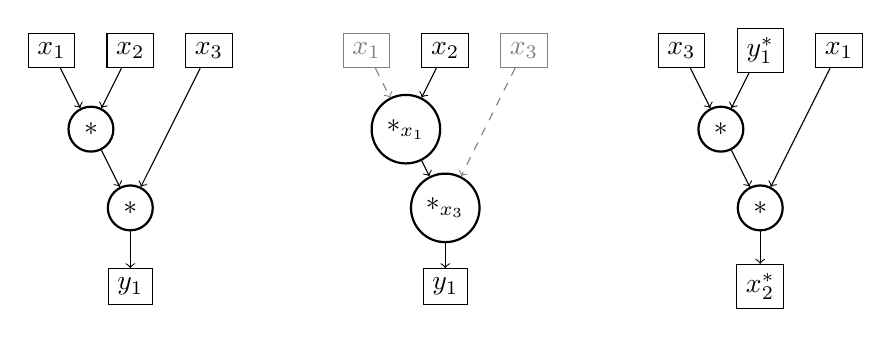
\begin{tikzpicture}
      \tikzstyle{node}=[circle,thick,draw=black,minimum size=4mm]
      \tikzstyle{arg}=[rectangle,thin,draw=black,minimum size=4mm]
      \tikzstyle{nodeg}=[circle,thick,draw=gray,minimum size=4mm]
      \tikzstyle{argg}=[rectangle,thin,draw=gray,minimum size=4mm]
      
      \begin{scope}
        \node[arg](in1){$x_1$};
        \node[arg,right of=in1](in2){$x_2$};
        \node[arg,right of=in2](in3){$x_3$};
        \node[node,below of=in1,xshift=5mm](times1){$*$};
        \node[node,below of=times1,xshift=5mm](times2){$*$};
        \node[arg,below of=times2](out){$y_1$};
        
        \path[->]
        (in1) edge (times1)
        (in2) edge (times1)
        (times1) edge (times2)
        (in3) edge (times2)
        (times2) edge (out);
      \end{scope}
      
      \begin{scope}[xshift=4cm]
        \node[argg](in1){\color{gray}{$x_1$}};
        \node[arg,right of=in1](in2){$x_2$};
        \node[argg,right of=in2](in3){\color{gray}{$x_3$}};
        \node[node,below of=in1,xshift=5mm](times1){$*_{x_1}$};
        \node[node,below of=times1,xshift=5mm](times2){$*_{x_3}$};
        \node[arg,below of=times2](out){$y_1$};
        
        \path[->]
        (in2) edge (times1)
        (times1) edge (times2)
        (times2) edge (out);
        
        \path[->,draw=gray,dashed]
        (in1) edge (times1)
        (in3) edge (times2);
      \end{scope}
      
      \begin{scope}[xshift=8cm]
        \node[arg](in1){$x_3$};
        \node[arg,right of=in1](in2){$y_1^\ast$};
        \node[arg,right of=in2](in3){$x_1$};
        \node[node,below of=in1,xshift=5mm](times1){$*$};
        \node[node,below of=times1,xshift=5mm](times2){$*$};
        \node[arg,below of=times2](out){$x_2^\ast$};

        \path[->]
        (in2) edge (times1)
        (times1) edge (times2)
        (times2) edge (out)
        (in3) edge (times2)
        (in1) edge (times1);
      \end{scope}
    \end{tikzpicture}  
  \end{center}

  \begin{itemize}
  \item Most applications require to \emph{linearize} a multi-linear
    program.
  \item Can we automatically deduce any possible linearisation of a
    program?
  \item \alert{Type inference systems can help us}
  \end{itemize}
\end{frame}

%%

\begin{frame}[fragile]
  \frametitle{Linearity inference}

  \begin{center}
    Suppose given a type \lstinline{R} implementing a ring. We want to
    define types \alert{\lstinline{L}} (for \emph{linear}) and
    \alert{\lstinline{S}} (for \emph{scalar}) such that the following
      equations hold
  \end{center}
  
  \begin{columns}
    \begin{column}{0.5\textwidth}
  \begin{semiverbatim}
    plus :: L -> L -> L
    plus :: S -> S -> S
  \end{semiverbatim}
    \end{column}
    \begin{column}{0.5\textwidth}
      \uncover<2>{\[\forall
        \alpha\in\{L,S\}.\alpha\ra\alpha\ra\alpha\]}
    \end{column}
  \end{columns}
  
  \begin{columns}[c]
    \begin{column}{0.5\textwidth}
  \begin{semiverbatim}
    times :: L -> S -> L
    \alt<2>{\st{times :: S {} -> L {} -> L}}{times :: S -> L -> L}
    times :: S -> S -> S
  \end{semiverbatim}
    \end{column}
    \begin{column}{0.5\textwidth}
      \uncover<2>{\[\forall
        \alpha\in\{L,S\}.\alpha\ra S\ra\alpha\]}
    \end{column}
  \end{columns}

  \begin{columns}
    \begin{column}{0.5\textwidth}
  \begin{semiverbatim}
    zero :: L
    zero :: S
  \end{semiverbatim}
    \end{column}
    \begin{column}{0.5\textwidth}
      \uncover<2>{\[\forall
        \alpha\in\{L,S\}.\alpha\]}      
    \end{column}
  \end{columns}

  \begin{columns}
    \begin{column}{0.5\textwidth}
  \begin{semiverbatim}
    one :: S
  \end{semiverbatim}
    \end{column}
    \begin{column}{0.5\textwidth}
    \end{column}
  \end{columns}
\end{frame}  

\begin{frame}[fragile]
  \frametitle{Linearity inference}
  
  \begin{center}
    The solution in Haskell
  \end{center}

  \begin{lstlisting}
    data L = L R
    data S = S R
    
    class Ring r where
      zero :: r
      (<+>) :: r -> r -> r
      neg :: r -> r
      (<*>) :: r -> S -> r

    one = S oneR
    (S a) == (S b) = a == b
  \end{lstlisting}

  \begin{center}
    To treat \alert{\lstinline{times :: S -> L -> L}}, we extend the
    Hindley-Milner type inference to handle lists of acceptable
    unifications.
  \end{center}
\end{frame}

%%
{\setbeamertemplate{navigation symbols}{}
\begin{frame}
  \frametitle{\tALpy{}\footfullcite{df+schost10}}
  
  \begin{block}{We are implementing}
    A Python-like ad-hoc language, compiled/interpreted in Python,
    featuring:
    \begin{itemize}
    \item Algebraic constructs (Rings, Modules, Fields, \ldots);
    \item Transposition of multilinear/recursive code;
    \item Parameterizable linearity inference (including commutative
      multiplication);
    \item Algebraic complexity preserving;
    \item Easily used on top of Computer Algebra Systems that have a
      Python interface;
    \item Other Computer Algebra Systems will be able to work with it
      as we will add more languages to the output of the compiler
      (OCaml and Haskell look easy, C is somewhat harder).
    \end{itemize}
  \end{block}

  \begin{center}
    \url{http://transalpyne.gforge.inria.fr/}
  \end{center}
\end{frame}
}

%%

\begin{frame}
  \frametitle{Perspectives}
  
  \begin{block}{Coding}
    Integration of automatic transposition in a Computer Algebra
    System. (Sage?  Mathemagix?)
  \end{block}

  \begin{block}{Arithmetic circuits and categorical semantics}
    Joint work with M. Boespflug:
    \begin{itemize}
    \item We have implemented a Domain Specific Language in Haskell,
    \item the result is not satisfactory due to Haskell's lack of
      support for dependent types.
    \end{itemize}
  \end{block}

  \begin{block}{Automated Theorem Provers}
    We plan to write a library to ease the use of the transposition
    principle in Automated Theorem Provers. (Coq? Agda? Isabelle?)
  \end{block}
\end{frame}

%%
%%

\section{Artin-Schreier towers}

\begin{frame}
  \frametitle{Newton sums}

  \begin{block}{Newton identities}
    \begin{itemize}
    \item Given a polynomial $\;f = \prod_j(X-\alpha_j)\in\K[X]$,
    \item The Newton sums are the $\;p_i = \sum_j\alpha_j^i\;$ for any $\;i\ge0$
    \end{itemize}
    \[\frac{f'}{f} = \sum_{i\ge0}\frac{p_i}{T^{i+1}} 
    \qquad\Leftrightarrow\qquad
    f = \exp\left(\int\frac{f'}{f}\right) = T^d\exp\left(-\sum_{i\ge1}\frac{p_i}{iT^i}\right)
    \text{.}\]
  \end{block}

  \pause

  \begin{block}{Trace formulas}
    Let $\algeb{A}=\K[X]/f(X)$, then
    \[p_i = \Tr_{\algeb{A}/\K}X^i\text{.}\] More generally for any
    $a,z\in\algeb{A}$, with $z$ primitive and $g$ its minimal
    polynomial
    \[\sum_{i\ge0}\frac{a\cdot\Tr_{\algeb{A}/K}z^i}{T^{i+1}} = 
    \sum_{i\ge0}\frac{\Tr_{\algeb{A}/K}az^i}{T^{i+1}} = \frac{A(T)}{g(T)}
    \qquad\text{and}\qquad
    a = \frac{A(z)}{g'(z)}
    \text{.}\]
  \end{block}
\end{frame}

%%

\begin{frame}
  \frametitle{Shoup's algorithm \parencite{shoup95,shoup99}}

  \begin{columns}
    \begin{column}{0.5\textwidth}
      \begin{center}
        \textbf{Polynomial evaluation}$:k[T]\ra\K/k$
        \[g\mapsto g(\sigma)\]
      \end{center}
    \end{column}
    \begin{column}{0.5\textwidth}
      \begin{center}
        \textbf{Power projection}$:(\K/k)^\ast\ra k[T]^\ast$
        \[\ell \mapsto \sum_{i>0} \frac{\ell(\sigma^i)}{T^i}\]
      \end{center}
    \end{column}
  \end{columns}

  \begin{block}{Power projection $=$ transposed polynomial evaluation}
    Let $\algeb{A}=\K[X]/f(X)$ and $z\in\algeb{A}$.  Take any
    algorithm that computes $g\mapsto g(z)$ and transpose it:
    \begin{itemize}
    \item Apply to $\Tr_{\algeb{A}/\K}$ to compute the characteristic
      polynomial of $z$;
    \item Apply to $a\cdot\Tr_{\algeb{A}/\K}$ to compute a
      representation of $a$ as a univariate polynomial in $z$.
    \end{itemize}
    The complexity of the original algorithm is preserved by the
    transposition principle!
  \end{block}

\end{frame}

%%

\begin{frame}
  \frametitle{Rational Univariate Representation}
  
  \begin{columns}
    \begin{column}{0.45\textwidth}
      \begin{block}{Generalization in many variables \parencite{giusti+lecerf+salvy01,rouiller99}}
        Let $\algeb{A} = \K[x_1,\ldots,x_n]/I$ and $z\in\algeb{A}$
        \begin{align*}
          g(z) &= 0\text{,}\\
          x_1 &= \frac{g_1(z)}{g(z)}\text{,}\\
          &\vdots\\
          x_n &= \frac{g_n(z)}{g(z)}\text{,}    
        \end{align*}
      \end{block}
    \end{column}
    \begin{column}{0.45\textwidth}
      \begin{block}{Change of basis}
        These two operations have the same cost, by the transposition
        principle:
        \begin{itemize}
        \item Going from the univariate basis
          \[\basis{Z} = \{1,z,\ldots,z^{d-1}\}\]
          to any basis $\basis{B}$ is equivalent to polynomial
          evaluation in $z$.
        \item Going from $\basis{B}$ to $\basis{Z}$ is equivalent to
          Rational Univariate Representation.
        \end{itemize}
      \end{block}
    \end{column}
  \end{columns}
\end{frame}

%%

\begin{frame}
  \frametitle{Application to towers of extension fields}
  
    \begin{columns}
    \begin{column}{0.3\textwidth}
      \Large\[\xymatrix{
        *+[r]{\U_k = \frac{\U_{k-1}[X_k]}{P_{k-1}(X_k)}}\ar@{-}[d]^p\\
        *+[r]{\U_{k-1}} \ar@{--}[dd]\\
        \\
        *+[r]{\U_1 = \frac{\U_0[X_1]}{P_0(X_1)}} \ar@{-}[d]^p\\
        *+[r]{\U_0 = \F_{p^d} = \frac{\F_p[X_0]}{Q(X_0)}}
      }\]
    \end{column}
    \begin{column}{0.65\textwidth}
      \begin{block}{Change of basis}
        $\basis{Z} = \{1,X_k,X_k^2,\ldots\}$
        $\basis{B} = \{1,X_{k-1},X_{k-1},\ldots,X_k,X_{k-1}X_k,X_{k-1}^2X_k,\ldots\}$
        \[
        \begin{cases}
          Q_{k}(X_{k})=0\\
          X_{k-1} = \frac{R(X_k)}{Q'_k(X_k)}\\
        \end{cases}
        \leftrightarrow
        \begin{cases}
          P_{k-1}(X_k,X_{k-1}) = 0\\
          Q_{k-1}(X_{k-1}) = 0
        \end{cases}\]
        \begin{itemize}
        \item Multiplication is faster on $\basis{Z}$;
        \item Embeddings are faster on $\basis{B}$;
        \item A fast algorithm for $\basis{Z}\ra\basis{B}$ implies a
          fast one for $\basis{B}\ra\basis{Z}$.
        \end{itemize}
      \end{block}
    \end{column}
  \end{columns}
\end{frame}

%%
{\setbeamertemplate{navigation symbols}{}
\begin{frame}
  \frametitle{Application to Artin-Schreir towers\footfullcite{df+schost09}}
  
  \begin{columns}
    \begin{column}{0.3\textwidth}
      \Large\[\xymatrix{
        *+[r]{\U_k = \frac{\U_{k-1}[X_k]}{P_{k-1}(X_k)}}\ar@{-}[d]^p\\
        *+[r]{\U_{k-1}} \ar@{--}[d]\\
        *+[r]{\U_1 = \frac{\U_0[X_1]}{P_0(X_1)}} \ar@{-}[d]^p\\
        *+[r]{\U_0 = \F_{p^d} = \frac{\F_p[X_0]}{Q(X_0)}}
      }\]
    \end{column}
    \begin{column}{0.65\textwidth}
      \begin{block}{Artin-Schreier extension}
        $\LK/\K$ of characteristic $p$ such that
        \[\LK=\K[X]/(X^p-X-\alpha)\text{.}\]
      \end{block}
      
      \begin{block}{Our construction}
        Let $\;x_0 = X_0\;$ such that
        $\;\Tr_{\U_0/\F_p}(x_0) \ne 0$, let
        \begin{align*}
          P_0 \quad&=\quad X^p - X - x_0\\
          P_i \quad&=\quad X^p - X - x_i^{2p-1}
        \end{align*}
        with $\;x_{i+1}\;$ a root of $\;P_i\;$ in $\;\U_{i+1}$.

        This tower is such that $x_i$ generates $\U_i/\F_p$.
      \end{block}
    \end{column}
  \end{columns}
\end{frame}
}

%%

\begin{frame}
  \frametitle{Application to Artin-Schreir towers}

  \begin{block}{The algorithms}
    All of these operations can be done in quasi-optimal time and
    space (w.r.t. the size of $\U_k$):
    \begin{itemize}
    \item Minimal polynomials of $x_i$ over $\F_p$ computed
      iteratively;
    \item Change $\basis{Z}\ra\basis{B}$ using a $p$-ary
      divide-and-conquer;
    \item Change $\basis{B}\ra\basis{Z}$ by trace formulas +
      transposed algorithms;
    \item Fast univariate multiplication via FFT, fast arithmetics
      (inversion, GCD, \dots);
    \item Traces and \emph{pseudotraces}, Frobenius morphisms;
    \item \alert{Isomorphisms with arbitrary Artin-Schreier towers via
      \cite{couveignes00}.}
    \end{itemize}
  \end{block}

  \begin{block}{Implementation}
    \begin{itemize}
    \item \texttt{C++} with \texttt{NTL} implementation released under
      GPL: \url{http://www.lix.polytechnique.fr/~defeo/FAAST/}
    \item Port to SAGE one day?
    \end{itemize}
  \end{block}
\end{frame}

%%
%%

\section{Isogenies}

\begin{frame}
  \frametitle{Isogenies between elliptic curves}
  
  \vspace{-2mm}

  {\large \[\I:E\to E'\]} \textbf{(Separable) isogeny}: (separable)
  non-constant rational morphism preserving the point at infinity.
  
  \begin{block}{Properties}
    \begin{itemize}
    \item Finite kernel, surjective (in $\clot{\K}$);
    \item Defined by rational fractions with a pole at infinity;
    \item $\card{E(\F_{q^n})} = \card{E'(\F_{q^n})}$ for every $n$,
    \item \emph{Dual} isogeny: $\;[m] = \I\circ\hat{\I}$.
    \end{itemize}
  \end{block}

  \vspace{-1mm}

  \begin{block}{
	\begin{overprint}
	\onslide<1> Multiplication	
	\onslide<2> Frobenius endomorphism
	\onslide<3> Separable isogeny, odd degree (simplified Weierstrass model)
	\end{overprint}
      }
    \begin{overprint}
      \onslide<1>
      \[\begin{aligned}
	{}[m] : E(\clot{\K}) &\rightarrow E(\clot{\K})\\
	                   P &\mapsto [m]P
      \end{aligned}\]
      $\ker\I = E[m], \quad\deg\I = m^2$.

      \onslide<2>
      \[\begin{aligned}
	\frob : E(\clot{\K}) &\rightarrow E(\clot{\K})\\
	               (X,Y) &\mapsto (X^q,Y^q)
      \end{aligned}\]
      $\ker\frob = \{\0\}, \quad\deg\I = q$.

      \onslide<3>
      \[\quad\I(X,Y) = \left(\frac{g(X)}{h^2(X)},
      cY\left(\frac{g(X)}{h^2(X)}\right)'\right)\]
      $\;\ell\;=\;\deg\I\;=\;
      \card{\ker\I} \;=\; 2\deg h + 1\;$ odd.
    \end{overprint}
  \end{block}
\end{frame}

%%


\begin{frame}
  \frametitle{Vélu formulas}
  
  \begin{block}{\cite{velu71} (algebraically closed field)}
    Given the kernel $H$, computes $\;\I : E\to E/H\;$ given by
    \begin{align*}
      &\I(\0_E) = \I(\0_{E/H})\text{,}\\
      &\begin{aligned}
        \I(P) = \Biggl(x(P) + \sum_{Q\in H^\ast}x(P+Q) - x(Q),
        y(P) + \sum_{Q\in H^\ast}y(P+Q) - y(Q) \Biggr) \text{.}
      \end{aligned}
    \end{align*}
  \end{block}

  \begin{block}{For $p\ge 3$, given $h(x)$ vanishing on $H$}
    {\footnotesize
      \[
      y^2 = f(x)
      \qquad
      t = \sum_{Q\in H^\ast} f'(Q)\text{,}
      \quad
      u = \sum_{Q\in H^\ast} 2f(Q)\text{,}
      \quad
      w = u + \sum_{Q\in H^\ast} x(Q)f'(Q)\text{,}\]}
    \[\alert{\I(x,y) = \left(\frac{g(x)}{h(x)}, y\left(\frac{g(x)}{h(x)}\right)'\right)}
    \quad\text{avec}\quad
    \frac{g(x)}{h(x)} = x + t\frac{h'(x)}{h(x)} - u\left(\frac{h'(x)}{h(x)}\right)'\]
  \end{block}
\end{frame}

%%


\begin{frame}
  \frametitle{Isogeny computation}
  
  \vspace{-1mm}

  \begin{center}
    \large
    Given $E, E', \ell$, compute $\I:E\to E'$
  \end{center}

  By Vélu formulas:
  $\I(x,y) = \left(\frac{g(x)}{h(x)}, cy\left(\frac{g(x)}{h(x)}\right)'\right)$,
  hence
  \[c^2(x^3 + ax + b){\left(\frac{g(x)}{h(x)}\right)'}^2 =
  \left(\frac{g(x)}{h(x)}\right)^3 + a'\frac{g(x)}{h(x)} + b'\]
  
  \vspace{-1mm}

  \begin{block}{BMSS algorithm \parencite{bostan+morain+salvy+schost08}}
    \begin{enumerate}
    \item Change variables $ S(x) =
      \sqrt{\frac{h(1/x^2)}{g(1/x^2)}} \quad\Leftrightarrow\quad
      \frac{g(x)}{h(x)} = \frac{1}{S(1/\sqrt{x})^2}$;
    \item Power series solution of 
      $\;c^2(bx^6 + ax^4 + 1){S'}^2 = 1 + a'S^4 + b'S^6$;
    \item Inverse the change of variables, reconstruct a rational
      fraction.
    \end{enumerate}
  \end{block}

  \vspace{-1mm}

  \begin{block}{\cite{lercier+sirvent08}}
    When $p$ exceeds the precision, a division by zero happens:
    \begin{itemize}
    \item Lift $E$ and $E'$ in the $p$-adics while keeping $\Phi_\ell\left(j(\tilde{E}),j(\tilde{E}')\right)=0$;
    \item Apply BMSS in $\Q_q$.
    \end{itemize}
  \end{block}
\end{frame}

%%

{
\setbeamertemplate{navigation symbols}{}
\begin{frame}
  \frametitle{Couveignes' algorithms}
  
  \begin{center}
    \textbf{Idea:} Send $E[p^k]$ over $E'[p^k]$
  \end{center}

  \begin{columns}[t]
    \begin{column}{0.5\textwidth}
      \centering\cite{couveignes94}

      \begin{uncoverenv}<2->
        \begin{itemize}
        \item Work in the formal group $\mathcal{E}$ of $E$: a
          \emph{formal point} is a series in a formal parameter
          $\;\tau$;
        \item Fix a precision \emph{large enough} for
          $\;\F_q[[\tau]]$ ($\sim\log_p4\ell$);
        \item Compute a morphism $\mathcal{U}(\tau) : \mathcal{E}
          \to \mathcal{E}'$;
        \item Reconstruct a rational fraction $\;\frac{g(X)}{h(X)} =
          \frac{1}{\mathcal{U}(1/X)}$;
        \item If $\frac{g}{h}$ is an isogeny, done; otherwise pick
          another $\mathcal{U}$.
        \item<3> $\mathcal{U}$ is uniquely determined by it action on
          $\;\mathcal{E}[p^k]\;$ for every $\;k$.
        \end{itemize}
      \end{uncoverenv}
    \end{column}
    \begin{column}{0.5\textwidth}
      \centering\cite{couveignes96}
      
      \begin{itemize}
      \item Compute the extensions $\U_i/\F_q$
        such that $E[p^i]$ is defined in $\U_i$;
      \item Pick $\;k\;$ \emph{large enough} ($k\sim\log_p4\ell$);
      \item Compute $\;P$, a generator of $\;E[p^k]$;
      \item Compute $\;P'$, a generator of $\;E'[p^k]$;
      \item Compute the polynomial $\;T\;$ vanishing $\;E[p^k]$;
      \item Interpolate $\;A : x(P) \mapsto x(P')$;
      \item Reconstruct a rational fraction  $\;\frac{g}{h}\equiv A \bmod T$;
      \item If $\frac{g}{h}$ is an isogeny, done; otherwise pick another $P'$.
      \end{itemize}
    \end{column}
  \end{columns}
\end{frame}
}

%%
{\setbeamertemplate{navigation symbols}{}
\begin{frame}
  \frametitle{Fast \cite{couveignes96}\footfullcite{df10}}

  \begin{tabular}{m{0.45\textwidth} m{0.45\textwidth}}
    $\bullet$ Compute the extensions $\U_i/\F_q$
    such that $E[p^i]$ is defined in $\U_i$; & \uncover<2->{An Artin-Schreir tower: $\tildO(\ell)$}\\
    $\bullet$ Pick $\;k\;$ \emph{large enough} ($k\sim 4\ell$); & \\
    $\bullet$ Compute $\;P$, a generator of $\;E[p^k]$; & \uncover<3->{An isomorphism of Artin-Schreier towers: $\tildO(\ell)$}\\
    $\bullet$ Compute $P'$, a generator of $\;E'[p^k]$; & \uncover<3->{An isomorphism of Artin-Schreier towers: $\tildO(\ell)$}\\
    $\bullet$ Compute the polynomial $\;T\;$ vanishing $\;E[p^k]$; & \\
    $\bullet$ Interpolate $\;A : x(P) \mapsto x(P')$; & \uncover<4->{Fast interpolation in towers of extensions: $\tildO(\ell)$}\\
    $\bullet$ Reconstruct a rational fraction  $\;\frac{g}{h}\equiv A \bmod T$; & \uncover<5->{XGCD: $\tildO(\ell)$}\\
    $\bullet$ If $\frac{g}{h}$ is an isogeny, done; otherwise pick another $P'$. & \uncover<6->{Repeat $O(\ell)$ times} \\
  \end{tabular}
\end{frame}
}
%%

\begin{frame}
  \frametitle{How to recognize an isogeny?}

  \begin{itemize}
  \item \textbf{Degree}: $\frac{g}{h}$ with $\deg g=\ell$, $\deg h = \ell-1$;\hfill\alert{$O(1)$}
  \item \textbf{Square factor:} $h = \prod_{Q\in H^\ast}(X- x(Q)) = f^2\;$ if $\ell$ odd;\hfill$\tildO(\ell)$
  \item \textbf{Group action:} Test with random points;\hfill$O(\ell)$
  \item \textbf{Factor of the $\ell$-division polynomial:} Compute $\phi_\ell\bmod h$.\hfill$\tildO(\ell)$
  \end{itemize}
\end{frame}

%%

\begin{frame}
  \frametitle{How to recognize an isogeny?}
  
  \[AU_i + TV_i = R_i  \qquad\Leftrightarrow\qquad  A\equiv \frac{R_i}{U_i} \bmod T\]
  \[\ell = 11\]
  \pause
  \begin{center}
  \begin{tabular}{c | c}
    $\deg R_i$ & $\deg U_i$ \\
    $3141592653589793238462643$ & 0 \\
    \pause
    \alt<7>{\textcolor{blue}{$3141592653589793238462642$}}{$3141592653589793238462642$} & 1 \\
    \pause
    $3141592653589793238462641$ & \alt<7>{\textcolor{blue}{$2$}}{$2$} \\
    \pause
    \vdots & \vdots\\
    $3141592653589793238462634$ & $9$ \\
    \pause\pause
    \Huge\alert{$11$} & \Huge\alert{$10$}\\
    \pause
    $10$ & $3141592653589793238462633$\\
    \vdots & \vdots
  \end{tabular}
  \end{center}
\end{frame}

%%

\begin{frame}
  \frametitle{Isogenies of unknown degree}
  
  \begin{itemize}
  \item This pattern is extremely rare.
  \item This is the only phase of Couveignes' algorithms that depends on $\ell$.
  \item<2-> \large Actually, this does not really depend on $\ell$,
    just on the existence of a \emph{gap}.
  \item<2-> \large If $\ell$ is not known in advance, it is enough to
    look for a \emph{gap}.
  \item<2-> \large Thus, any isogeny of degree $\ll p^k$ can be
    obtained with one single run of Couveignes' algorithms.
  \end{itemize}  
\end{frame}

%%

\begin{frame}
  \frametitle{Perspectives}
  
  \begin{block}{Looking for the quasi-linear complexity}
    \begin{itemize}
    \item The Weierstrass model has a canonicity defect: use other parameterizations? Formal groups?
    \item How to obtain \emph{local} information on the behavior of
      the isogeny? (for example, its action on $E[p]$)
    \end{itemize}
  \end{block}

  \begin{block}{Isogenies of unknown degree}
    \begin{itemize}
    \item This variant of \cite{couveignes96} is at the moment the
      fastest (both in theory and in practice) algorithm for this
      task.
    \item We tested two curves over $\F_{2^{161}}$, isogenous of
      unknown degree, taken from \cite{teske06};
    \item Certified in 258 cpu-hours that no isogeny of degree
      $2^c\ell$ for any $c$ and $\ell<2^{11}$ exists;
    \item Certified in 1195 cpu-hours that no isogeny of
      degree les then $2^{12}$ exists.
    \item The two curves have an isogeny of (very smooth) degree $\sim
      2^{1050}$. Proving that no isogeny of smaller degree  exists
      is momentarily out of reach.
    \end{itemize}
  \end{block}
\end{frame}

%%

\begin{frame}
  \frametitle{Z'en voulez plus?}
  
  \begin{center}
    \Large Fast Algorithms for Towers of Finite Fields and Isogenies

    \bigskip

    \large 13 décembre, École Polytechnique

    \normalsize heure et amphi à préciser
  \end{center}
\end{frame}

%%
%%

{\setbeamertemplate{navigation symbols}{}
\begin{frame}[allowframebreaks]
  \frametitle{References}

  \defbibfilter{books}{\type{book} \or \type{booklet} \or \type{thesis}
    \or \type{report} \or \type{collection} \or \type{manual}
    \or \type{periodical} \or \type{proceedings}}
  \defbibfilter{articles}{\not \(\type{book} \or \type{booklet} \or \type{thesis}
    \or \type{report} \or \type{collection} \or \type{manual}
    \or \type{periodical} \or \type{proceedings}\)}

  \beamertemplatebookbibitems
  \printbibliography[filter=books]
  \beamertemplatearticlebibitems
  \printbibliography[filter=articles]
\end{frame}
}
\end{document}


% Local Variables:
% mode:flyspell
% ispell-local-dictionary:"american"
% mode:TeX-PDF
% mode:reftex
% End:
%
% LocalWords:  Isogeny abelian isogenies hyperelliptic supersingular Frobenius
% LocalWords:  isogenous
